\chapter{Evaluation}
We followed Pol, Koomen and Spillner's way of testing \cite{pol2000management} by using their model and dividing the process of testing into the 
six phases planning, preparation, test-specification, execution and result analysis. Due to extent this work is aimed at, 
it was not feasible to implement all the systems of the related solutions on this field on a common environment
to get a fair assessment for each work and to really estimate how each solution performes against the others. 
On the other hand such a comparison would have to be treated with caution since, each solution is designed with another metric/goal kept in mind.
\cite{overview_caa} attempts to cover and compare the current most famous solutions on \ac{CA}. 
Therefore the following tests will focus on the comparison between AutoWDS basic and its extended, optimized version.
Furthermore our tests were restricted to the evaluation of spanning tree topolgies, because as AutoWDS currently 
still uses a briged network for its accesspoints instead of a fully grown routing system, with the drawback of \ac{STP} being active.
This means even if we would try to run a network topology with survival paths in it on AutoWDS, \ac{STP} would disable some links in order to 
eliminate circles in the topology \footnote{Circles in a network topology are undesired since they can create broadcast-storms See IEEE 802.1D}.
As a consequence achievable throughput will be lower than it could be with survival paths.

\newpage

  \section{Planning}
    The goal of this test is to confirm the claim of an increase in overall throughput of AutoWDS extended compared to AutoWDS basic.
    Therefore we will evaluate the whole process by deploying an actual WDS with AutoWDS instead of just performing a code analysis or review.
    To discern performance gains we run AutoWDS basic and extended on the same networking setup and measure its achieving overall throughput.
    In order to create enough throughput we attach traffic generators to the accesspoints to simulate real clients.
    These generators will then send data to all the other nodes in the network.
    To get the values of how much data was actually carried over the wireless network, we will query the accesspoints for this information in a way that it 
    does not affect the measurement, like querying too often for too much data would cause additional load on the APs and network.
    
    The scope of the test is deliberately kept to the same scale as portrayed in the requirements analysis.
    That means it will not exceed 100 accesspoints with expected target size of about 30 devices.
    We would expect to recognise noticeable differences between the two systems, since interference was strongly avoided where possible and radio modules 
    are more efficiently used than before.
    
    We would expect a significant increase of data that has been able to transmit due to the usage of multiple collision domains the same one could
    expect by comparing a network hub, which has essentially just one collision domain and a network switch which has multiple domains and does not have
    to wait until the medium is free for sending again. The second source for an increased throughput would be the number of packets that could be received
    without errors due to interference.
    
    \begin{figure}[h!]
      \centerline{
	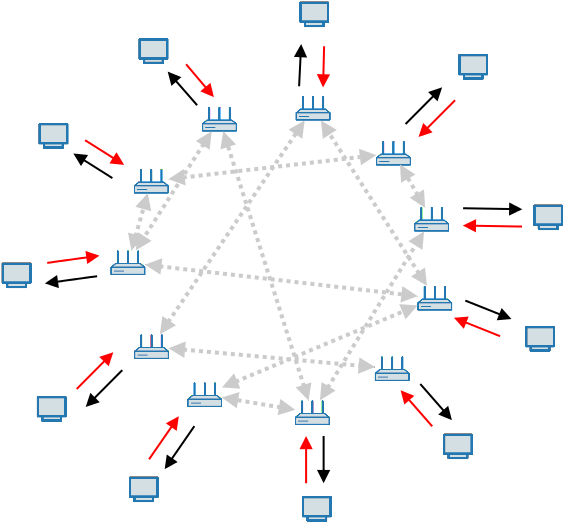
\includegraphics[width=0.6\textwidth]{figures/testsetup_logic}
	\caption{Concept of testbed with traffic-generating systems attached to APs by cable, sending broadcast traffic and saturating the network.}
      }
      \label{fig:testsetup_logic}
    \end{figure}    
    
  \section{Preparation}
    The basic approach for measuring the throughput is to attach traffic generators to the accesspoints and make those send as much broadcast traffic to all
    other stations which are part of this network and therefore saturate the throughput capabilities of the network. 
    The idea behind this setup is to simulate real end-device-clients attached to the accesspoints, where each client has its own ip address and 
    therefore mac- address and table. Cabling the clients to the accesspoint instead of using real mobile devices like smartphones was preferred as this gave
    us more control to keep out other impacting effects and moving around 3 Devices per AP would have been a challenge, especially to do it in the same
    way for each test-run to keep circumstances reproducible.
    
    Due to limitations in cabling for power and network and severe interference in 
    certain parts of our building we could not use the 30 accesspoints as initially planned.
    Therefore we had to consider ourselves satisfied with 12 accesspoints.
    
    \subsection{Modifications for the Test}
      Although we did not have to modify the code for the network, we had to change some small details in the LCOS firmware to better fit the data we needed as input for
      the algorithms to our requirements. Therefore we took the latest stable firmware version 9.0 and added some special extension.
   
\newpage
   
    \subsection{Physical Structure}
      We deployed the accesspoints at a typical office environment as depicted in \ref{fig:2ndfloor} and used only omnidirectional antennas for the accesspoints.
      Additionally the APs were also connected by wire to their client systems on a central server in form of virtual machines.
      
      \begin{figure}[h!]
	\centering
	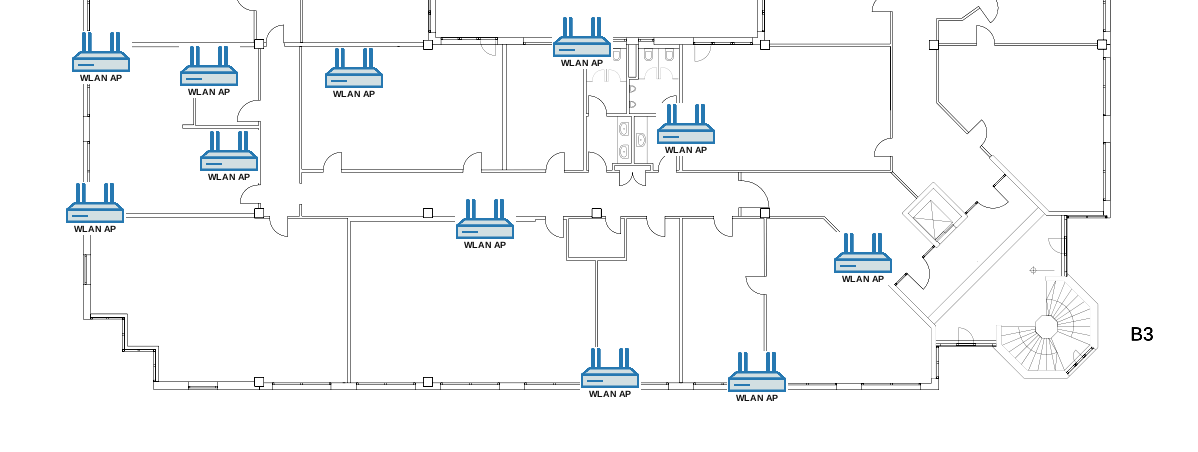
\includegraphics[width=\columnwidth]{figures/Lancom-flur-withaps}
	\caption{Physical arrangement of accesspoints in a typical office complex spread over an area of rougly 15m x 40m}
	\label{fig:2ndfloor}
      \end{figure}
      
      The hardware we used were mainly LANCOM devices and also 6 OpenBAT devices, although flashed with the same firmware.
     
      List of used hardware:
      \begin{itemize}
	\item 3 x LANCOM L322agn dual Wireless \cite{lancom}
	\item 3 x LANCOM L-452agn dual Wireless
	\item 6 x Hirschmann OpenBAT-R
	\item 1 x LANCOM WLC-4100
	\item 2 x LANCOM GS-2352P
      \end{itemize}
      
      Note that the distance between the accesspoints should have been increased even further to more closely resemble a real usecase-deployment.
      Thus the actual interference would have gone up, since with a lower Signal to Noise ratio the APs would not be able to recognize each others 
      transmissions as those and categorize it as interference instead of applying CSMA/CD, leading to more corrupt packets.
      We were able to simulate this problem with a reduced transmit-power,
      but even on the lowest setting most of the accesspoints were still able to receive each others beacons. 
      This is another factor that will lower the throughput we will notice in the testresults for the optimized scenario.
      Therefore the throughput-differences between the two systems in a real deployment will probably be higher, since the basic AutoWDS will perform worse.
    
    \subsection{Logical Structure}
      We simulated the traffic generating systems with OpenVZ \cite{openvz} on one server with a VLAN for each system to separate the traffic for each client.
      This was done so that we did not need to setup twelve different real hardware machines as those merely have to generate and receive traffic.
      The VLAN infrastructure is completely transparent to the VZ containers and the accesspoints since the host-machine on the server 
      encapsulates all frames before sending if over the VLAN Trunk to the switch, which again decapsulates the frames before sending them to the accesspoints.
      
      \begin{figure}[h!]
	\centerline{
	  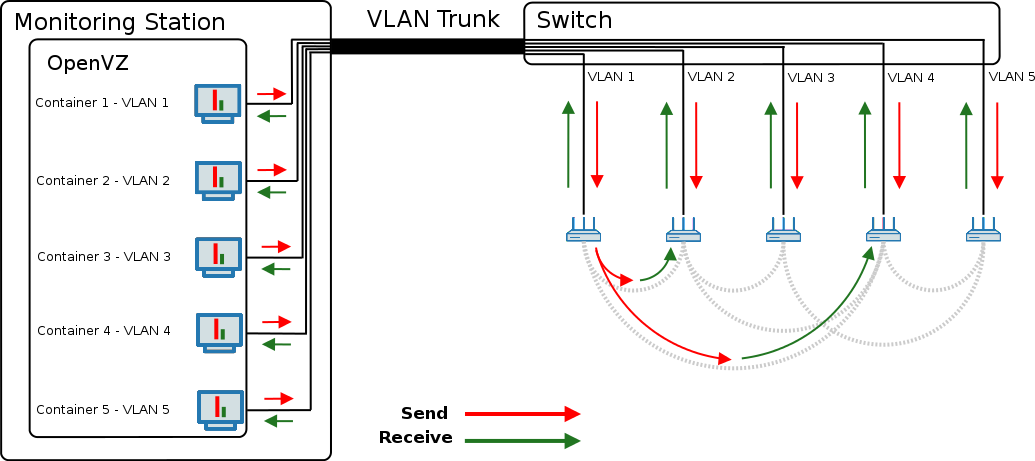
\includegraphics[width=1\textwidth]{figures/testsetup_openvz}%
	  \caption{Test arrangement with OpenVZ and VLANs to simulate a busy network.}
	}
	\label{fig:testsetup_openvz}
      \end{figure}
      
      To generate the traffic we used IPerf \cite{iperf} on the attached systems in UDP mode with a datarate of 1Mbit per second for a total of 10 Minutes.
      Since we could not directly send UDP frames to broadcast addresses with iperf, we ran multiple instances of iperf with different target ip addresses.
      Although 1Mbit for each stream may not seem much, but after multiplying it with the number of targets and the up- and downstreams the effective rate results in
      1Mbit * 12 * 2 = 24Mbit/s for each accesspoint. As we will see later on, this will turn out to be enough to completely saturate the wireless network but is still within
      the capabilities of the used Gigabit Ethernet to get the data to and from the accesspoints, 
      as 24Mbit/s * 11 = 264Mbit/s does not exceed the 1000Mbit/s VLAN Trunk connection as possible bottleneck.
      
      \begin{listing}[h!]
	\begin{lstlisting}
iperf -u -c 172.16.40.2* -t 600 -b 1M
	\end{lstlisting}
	\caption{IPerf mode of operation for generating the traffic.}
	\label{lst:iperf}
      \end{listing}
    
  \section{Specification}
    Each test run describes a 10 minutes performance stress test for the network with throughput saturation. 
    This should be enough time to notice any temporal effects and to get a picture of the lasting performance.
    
    To keep environmental conditions for each of the AutoWDS systems as similar as possible we conducted the runs alternatively with respect to channel usage.
    So that a possible additional temporal interference in a certain band would affect both runs and not just favor a single system.
  
    Actually to get more statistic significance we should have run this test-array more than once, but as for each new setup there had to 
    be invested a considerable amount of time in the pre-setup of AutoWDS (getting it up and running, despite a few bugs), this was not feasible within
    the timeframe that was scheduled to execute the whole evaluation.
    
    Additionally we ran the testcases with two different antenna power-settings to simulate the hidden station problem. Therefore we first set the radios to full power 
    resulting in a high connectivity between the nodes and on a second run decreased the transmit power as much as possbile to get a network with a smaller degree
    of interconnectivity.
  
    \begin{table}[h!]
      \centering
      \begin{tabular}{clll}
	Testrun nr. & AutoWDS version & Channels used & Antenna power\\ \hline
	1 & basic & 1 & low \\
	2 & extended & 1,6,11 & low \\
	3 & basic & 36 & low \\
	4 & extended & 36,40,44 & low \\
	5 & basic & 1 & high \\
	6 & extended & 1,6,11 & high \\
	7 & basic & 36 & high \\
	8 & extended & 36,40,44 & high \\
	9 & extended & 1,6,11,36,40,44 & low \\
	10 & extended & 1,6,11,36,40,44 & high \\
      \end{tabular}
      \caption{Testruns executed with different Channelusage and varying antenna power.}
      \label{tab:testruns}
    \end{table}
    
\newpage
    
  \section{Execution}
    The tests were executed mainly in the evening and on weekends in order to catch timeframes where the radio bands are not as crowded as on an ordinary workday.
    The general procedure for a testrun was implemented as follows:
    \begin{enumerate}
      \item Power on the System (WLC + APs).
      \item Wait until all accesspoints are connected to the wireless backbone (See description of AutoWDS at \ref{autowdsbasic})).
      \item For AutoWDS basic continue with next step, for the extended version also the following additional steps have to be conducted.
	\begin{enumerate}
	 \item Wait until all the wireless measurements arrived at the \ac{WLC}.
	 \item Run our algorithm, which reads data from the WLC, computes a solution and writes back the topology-to-do to the WLC.
	 \item Wait until the WLC reconfigured all the accesspoints.
	 \item Wait until the APs all successfully reconnected through their new connections to the wireless backbone.
	\end{enumerate}
      \item Start the scripts that iteratively query the APs for their status tables every 7 seconds.
      \item Start the receiving iperf processes on the VZ machines.
      \item Start the sending iperf processes on the VZ machines.
      \item Wait the predefined 10 minutes until the tests finish.
      \item Archive the collected data.
    \end{enumerate}
    
\newpage

    During the testruns we made some snapshots of the network topolgies, where you can clearly see the improvements.    
    \begin{figure}[h!]
      \centering
	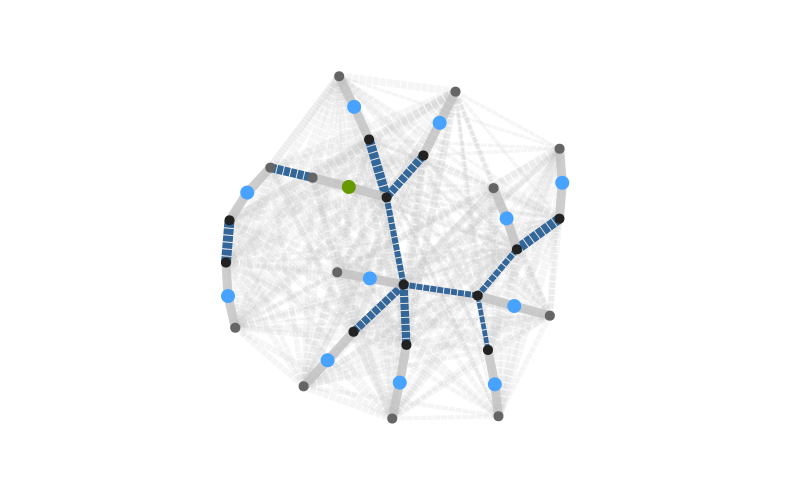
\includegraphics[width=\textwidth]{figures/topo_chan_1}%
	\caption{Topology of the testnetwork with only one channel in use (AutoWDS basic).\protect\footnotemark }
      \label{fig:topo_chan_1}
    \end{figure}
    
    \footnotetext{Different edge-colors indicate different channels. Also edge thickness denotes the quality of a link, where thicker means higher quality.}

    \begin{figure}[h!]
      \centerline{
	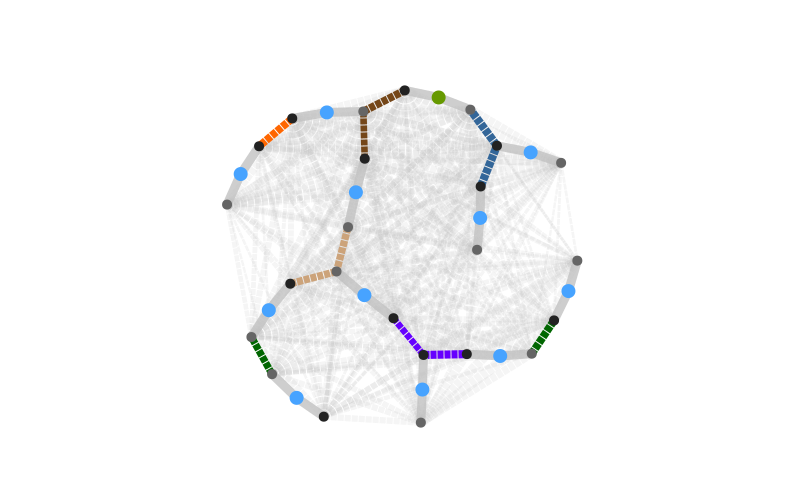
\includegraphics[width=\textwidth]{figures/topo_chan_1_6_11_36_40_44}%
	\caption{Topology of the testnetwork with six channels in use (AutoWDS extended).}
      }
      \label{fig:topo_chan_1_6_11_36_40_44}
    \end{figure}
    
\newpage
    
    After gathering all the archived data from the testruns and aggregating those, we receive the following picture.
    
    \begin{figure}[h!]
      \centerline{
	\includegraphics[width=0.62\textwidth]{figures/TestDataDiagramme/20/rx_bytes}%
	\includegraphics[width=0.38\textwidth]{figures/TestDataDiagramme/20/rx_bytes_boxplot}%
      }
      \caption{Received bytes with decreased antenna transmit power}
      \label{fig:rx20_bytes}
    \end{figure}
    
    \begin{figure}[h!]
      \centerline{
	\includegraphics[width=0.62\textwidth]{figures/TestDataDiagramme/3/rx_bytes}%
	\includegraphics[width=0.38\textwidth]{figures/TestDataDiagramme/3/rx_bytes_boxplot}%
      }
      \caption{Received bytes with full transmit power}
      \label{fig:rx3_bytes}
    \end{figure}
    
    Analyzing the successfully received bytes for the low power \ref{fig:rx20_bytes} and high power \ref{fig:rx3_bytes} setup we recognize noticeable differences for 
    each channel-assigning.
    
      \begin{itemize}
	\item The base scenarios where only one channel was utilized performe the worst within a range of 0.5 to 1.5Mbit/s on average per accesspoint.
	  Using three channels gives roughly three times the throughput (2.5 - 5Mbit/s for 2.4Ghz and 2.5 - 5Mbit/s for 5Ghz) compared to the baseline.
	  Utilizing up to 6 Channels shows the best results with an effective throughput of 5.5 - 9Mbit/s. Note that the gain for the 6 channel setup 
	  is still linear as it provides roughly 6 times the throughput of the baseline.
	\item We further discern that the high transmit power setup outperformes the low power setup by a factor of two with an even more noticeable difference.
	\item With slight variations for the high-power 3/2.4Ghz setup the rates are also rather constant.
	\item Besides the high-power 1/5Ghz setup we realize 5Ghz's superiority over the 2.4Ghz band.
      \end{itemize}

    \begin{figure}[h!]
      \centerline{
	\includegraphics[width=0.56\textwidth]{figures/TestDataDiagramme/3/recpackerr}%
	\includegraphics[width=0.44\textwidth]{figures/TestDataDiagramme/3/recpackerr_boxplot}%
	\caption{Ratio of successfully received packets to packets containing errors for reduced transmit power scenario}
      }
      \label{fig:3recpackerr}
    \end{figure}
    \begin{figure}[h!]
      \centerline{
	\includegraphics[width=0.56\textwidth]{figures/TestDataDiagramme/20/recpackerr}%
	\includegraphics[width=0.44\textwidth]{figures/TestDataDiagramme/20/recpackerr_boxplot}%
	\caption{Ratio of successfully received packets to packets containing errors for full transmit power scenario}
      }
      \label{fig:20recpackerr}
    \end{figure}
    
\newpage
    
    From the existing data we could also extract the number of errors over time. Deriving the rate and setting those in proportion to
    successfully and hence all transmitted packets we can now take a look at the effective rate of corrupt packets and therefore bytes as an error in a packet 
    spoils the whole packet and all data in it.
    \begin{itemize}
      \item The base-scenarios again perform subpar and show the highest error rates with 10 to 65 percent depending on the transmit power.
	Using three channels the error-rates shrink to 6 to 30 percent.
	Adding another three channels seems to further reduce error rates to 5 to maximal 10 percent.
      \item As with the successfully transmitted bytes we note a greater difference when using different transmit power setups. 
	Increasing the transmission power also increases the error-rates at least twice and up to 6 times (one channel/ 2.4Ghz).
      \item In the low-power setup error-rates a rather constant compared to the high-power setup where we discern greater deviations especially for those tests in the 5Ghz band.
    \end{itemize}
    
    Note that different from \cite{pol2000management} recommendation the test was not run by someone impartial, but also by us.

  \section{Analysis}
    The results perfectly match our expectations, despite all the limitations of our testbed.
    Using only a single channel in AutoWDS basic does not scale well, no matter how much transmit power is used and independent of the band.
    Not only is the baseline scenario incapable of transmitting much data, most of it is also corrupt.
    The results also affirm our estimate that the basic version transfers little more than control data.
    
    While setting up the test environment we also noticed that this effect of medium overload is no result of the size of our network.
    Whereas two unimpeded accesspoints were able to achieve a throughput of about 2Mbit in each direction, adding a third one would dramatically 
    decrease overall throughput down to about 100kbit or less, growing worse with each newly added accesspoint in receive-range. 
    Even spreading the accesspoints further apart would not promise better results since the inherent problem of reusing the same channel for the forwarding and receiving 
    link restricts the forwarding capabilities rigorously.
     
    As the figures show, the outcome is dependent on the number of channels used as a setup with only three distinct channels allowed yields still better
    results than a mono-channel-setup but is inferior to a setup where we can use even more channels as this gives us the possibility to use more collision domains
    which results in more available bandwidth and therefore increased throughput. In our example we used accesspoints with only two radios, which
    limits us in selecting separate modules for different connections so that an accesspoint which already established two connections over its two modules
    would have to share one of its modules in order to apply a new link to a foreign accesspoint in order to maintain connectivity.
    This means instead of just using a lot of channels or just using a lot of radios per \ac{AP} a combination of both promises the best results.
    \begin{figure}[h!]
      \centerline{
	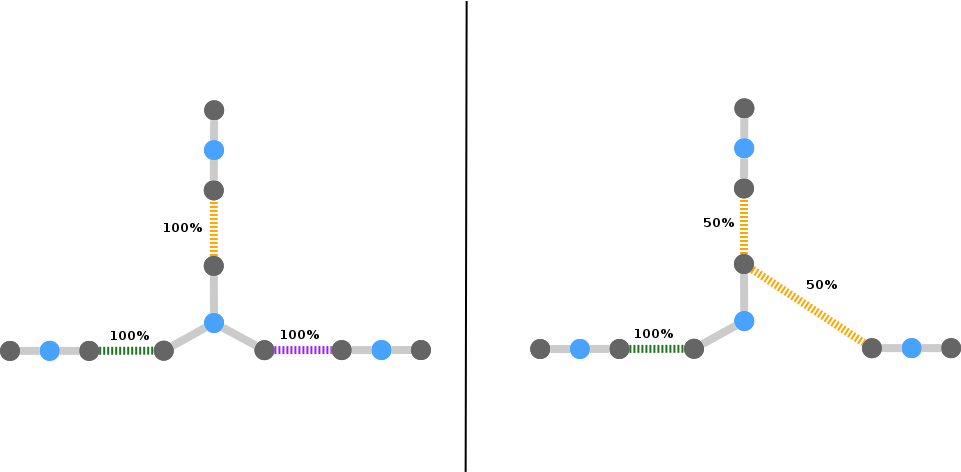
\includegraphics[width=0.56\textwidth]{figures/3modulesvs2}
	\caption{Link separation capability for an accesspoint with three modules compared to an accesspoints with two modules.}
      }
      \label{fig:3modulesvs2}
    \end{figure}
    
    Compared to the base scenario our link selection and channel assignment algorithm roughly doubles the throughput with every channel added. 
    Of course this effect is limited by using a separate channel for each link and also by the number of modules for an accesspoint 
    since the former effectively assigns each link its own channel and the latter is a question of practical relevance as current APs are only 
    shipped with two or a maximum of three radio modules. As our gathered data indicate, it is after all a notable improvement to utilize multiple channels and modules.
    
    \subsection{Reflection on the Requirements}
      In this section we will analyze by how far we were able to meet the imposed requirements and restrictions from the requirement analysis..
  
      \begin{description}
	\item [Increased Throughput:]
	  Our measurement results indicate that throughput could significantly be increased. How much is determined by the input parameters of the algorithms like
	  channels that can be utilized and hardware environments like the number of radio modules available at the accesspoints. 
	  
	\item[Reduced end-to-end Link Failures:]
	  The survival path property takes care of this requirement. That is for the given error-scenario of one failing connection at a time, there is always
	  a backup connection over a different link available as far as the underlying topology permits. As we were not able to test this feature 
	  with the given implementation we are nevertheless confident that also this requirement has been met.
	  If multi-flow / routing support will be implemented for our hardware in the future a decrease in node separation for failing links should be recognizable.
	  Therefore we also met the successfully met the requirement of a two-edge-connected network topology.
	  
	\item[Multiple Radios Utilized:]
	  Our algorithm utilizes the radio-modules as far as they are relevant for creating links between accesspoints with a high estimated throughput.
	  Depending on the given infrastructure not all radio modules are necessarily used, since not all of them are needed in order to create a connected network topology.
	  Moreover using all available links may not necessarily be beneficial, since if not enough radios are available, adding new links can force
	  other radios to the same channel, which effectively leads to sharing a single channel between more radios instead of exclusive access (See \ref{fig:lessismore}).
	  
	  \begin{figure}[h!]
	    \centerline{
	      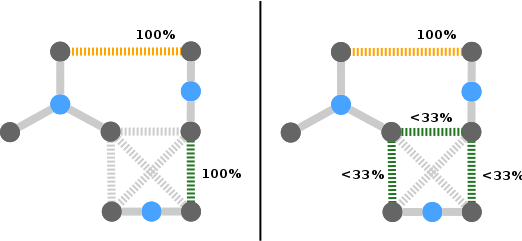
\includegraphics[width=0.56\textwidth]{figures/lessismore}
	      \caption{Adding additional links does not necessarily increase throughput performance.}
	    }
	    \label{fig:lessismore}
	  \end{figure}
	
	  Having some radio modules to spare gives us the opportunity to use those exclusively for client 
	  connections and assigning them a channel which does not interfere with the wireless backbone.
	  
	  \begin{figure}[h!]
	    \centerline{
	      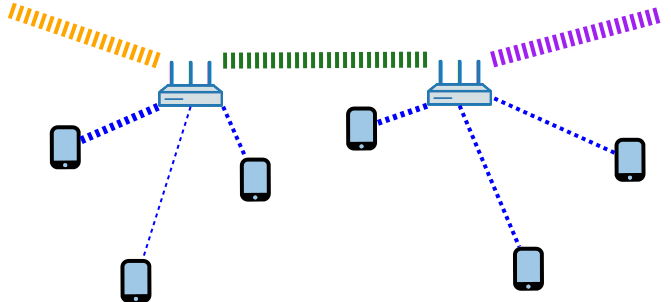
\includegraphics[width=0.56\textwidth]{figures/moduletospare}%
	      \caption{Unused modules can be used here for separate client connections without interfering the WLAN backbone.}
	    }
	    \label{fig:moduletospare}
	  \end{figure}
	
	\item[Capability of Using Variable Channelsets:]
	  Our algorithm selects channels from a given input set of channels. Only those channels are then used to determine the channel assignment.
	  It is even possible to specify only one channel, resulting in a topology optimized network graph only.
	  Therefore this solution also fullfills this requirement.  
	  
	\item[Centralized Computation and Configuration:]
	  The requirement dictates that computing a solution should be possible on a centralized entity (Servers/WLC).
	  Our algorithm was implemented as a python script and can be run on a single system if given the right input data.
	  Creating the configurations for the accesspoint will still be conducted by the central WLC as depicted in \ref{fig:dataflow}.
	  
	\item[Static Environment:]
	  Also the second requirement is taken into consideration, since our algorithm is specially designed for a static environment where link quality 
	  and linkstate stay the same for a foreseeable time.
	  If major changes in network connectivity or link quality occur the chosen network topology and channel assignment
	  may lead to temporal suboptimal results, therefore also a recomputation of the network topology would have to be triggered.
	  Currently there are no automatic triggers implemented, but planned in the future.
	  
	\item[Layer two Usage:]
	  Accesspoints use bridged point to point connections to span the wireless network backbone, therefore creating no obstacles for layer two frames.
	  The ethernet frames are just forwarded like in a switched environment and not encapsulated in layer three packets.
	  
	\item[Economic Restrictions:]
	  The Runtime of the algorithms is mainly dependent on the number of connections between the nodes. Calculating the initial spanning tree is done in BFS mode and 
	  therefore has quadratic runtime for the worst cast, depending on how sparse the graph is. The following calculation of the survival paths has also quadratic runtime 
	  since we iterate over all connections and for each connection in the worst case over all other connections to find the backup path. The channel assignment is then again
	  In a common deployment scenario the underlying network graph will be very sparsly connected since the number of accesspoints used and placement are carefully selected.
	  Mostly they are placed in a way that they span a network over an area as far as possible.
	  Current deployments and deployments in near future won't exceed 100 accesspoints. 
	  Even if fully meshed with a total of \(\sum \limits_{i=1}^{100} i = \frac{100(100+1)}{2}=5050\)
	  edges it won't pose a problem to the capabilities of a WLC or an administrators machine.
	  
      \end{description}
      
\newpage
      
    \subsection{Reflection on Related Work}
      Comparing our solution to those of others would need some common ground. For example hardware requirements, number of modules and in general heterogenity/homgenity of
      the network are factor that could play in favor of some algorithms and therefore won't lead to fair results. Additionally different solutions were designed to 
      achieve different goals like throughput, latency or weighted throughput networks. Certainly there we could agree on this common deployment and compare each solution for random
      networks with respect to throughput, but this would require a full-scale simulation as hardware-resources are limited and too easily prone to real world difficulties.
      Although maybe a key aspect of this work, we did not have enough time to simulate even our own solution and therefore neither those of others. Nevertheless we would appreciate
      if someone further work on this field. In order to at least provide some kind of comparison we will take a look at the features of our work, which 
      most of the related work did not show or provide.
      
      \begin{description}
	\item [Variables Nr. of Radios:] Our algorithms support a variable number of radios on each device instead of a fixed numer like in \cite{INSTC}. 
	  This allows to optimize the wireless network even for heterogeneous environments where devices have a variable number of radios or just one.
	\item [Vendor Neutral:] Although we used only LANCOM devices in our case, the solution is basically vendor neutral. As long as the devices provide the required data,
	  any network with devices that can be configured (also manually) to use a specific link for a certain radio can profit from out optimization.
	\item [No MAC changes:] Our solution does not require any \ac{MAC}-layer changes and can be run on any commodity \ac{WLAN} hardware.
	\item [No Forced Backup Links:] Thanks to out modular approach adding redundant links to the initial \ac{MST} is completely optional. 
	  You are free to only optimize and use MST if you are also limited by the STP like we were in our evaluation.
	\item [Considers Foreign Interference:] Admittedly we are not the first to do so (\cite{BFS-CA}), but our solution also considers foreign interfering WLANs which can have a great impact in performance
	  if those are neglected.
	\item [Customizable Survival Pats:] In order to create the redundant links (survival paths) we iterated over each link in the MST and simulate it failing.
	  You could just as well iterate over the nodes in the MST to get a \textit{k}-node-connected survival graph or whatever order you chose.
	  This means you can add redundant links in decreasing order of optimality up to a fully meshed graph.
	\item [Customizable Ranking-Formula:] Without great effort you can also adapt the ranking-formula and create a spanning tree which is optimal to some other metrics you need.
	\item [No Gateway/Special Node necessary:] At last you do not need a special gateway node like in \cite{BFS-CA} to start our algorithm with.
      \end{description}